\documentclass{standalone}
\usepackage{tikz}
\usetikzlibrary{decorations.pathreplacing}

\begin{document}

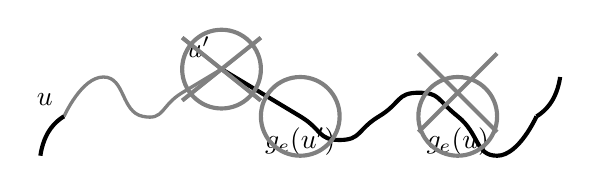
\begin{tikzpicture}

% Styles
\tikzstyle{every path}=[line width=1.5pt]

% Original walk in gray
\draw[gray, line width=1.2pt] plot [smooth, tension=1] coordinates {(-3,0) (-2.5,0.5) (-2,0) (-1.5,0.3) (-1,0.6)};

% Modified walk in black
\draw[black] plot [smooth, tension=1] coordinates {(-1,0.6) (-0.5,0.3) (0,0) (0.5,-0.3) (1,0) (1.5,0.3) (2,0) (2.5,-0.5) (3,0)};

% Curves at start and end
\draw[black] plot [smooth, tension=1] coordinates {(-3,0) (-3.2,-0.2) (-3.3,-0.5)};
\draw[black] plot [smooth, tension=1] coordinates {(3,0) (3.2,0.2) (3.3,0.5)};

% Labels
\node at (-1,0.6) [above left] {$u'$};
\node at (0,0) [below] {$g_e(u')$};
\node at (2,0) [below] {$g_e(u)$};
\node at (-3,0) [above left] {$u$};

% Circles
\draw[gray] (0,0) circle (0.5);
\draw[gray] (2,0) circle (0.5);
\draw[gray] (-1,0.6) circle (0.5);

% Diagonal lines
\draw[gray] (-1.5,1) -- (-0.5,0.2);
\draw[gray] (-1.5,0.2) -- (-0.5,1);
\draw[gray] (1.5,0.8) -- (2.5,-0.2);
\draw[gray] (1.5,-0.2) -- (2.5,0.8);

\end{tikzpicture}

\end{document}